% Options for packages loaded elsewhere
\PassOptionsToPackage{unicode}{hyperref}
\PassOptionsToPackage{hyphens}{url}
\PassOptionsToPackage{dvipsnames,svgnames,x11names}{xcolor}
%
\documentclass[
  letterpaper,
  DIV=11,
  numbers=noendperiod]{scrreprt}

\usepackage{amsmath,amssymb}
\usepackage{iftex}
\ifPDFTeX
  \usepackage[T1]{fontenc}
  \usepackage[utf8]{inputenc}
  \usepackage{textcomp} % provide euro and other symbols
\else % if luatex or xetex
  \usepackage{unicode-math}
  \defaultfontfeatures{Scale=MatchLowercase}
  \defaultfontfeatures[\rmfamily]{Ligatures=TeX,Scale=1}
\fi
\usepackage{lmodern}
\ifPDFTeX\else  
    % xetex/luatex font selection
\fi
% Use upquote if available, for straight quotes in verbatim environments
\IfFileExists{upquote.sty}{\usepackage{upquote}}{}
\IfFileExists{microtype.sty}{% use microtype if available
  \usepackage[]{microtype}
  \UseMicrotypeSet[protrusion]{basicmath} % disable protrusion for tt fonts
}{}
\makeatletter
\@ifundefined{KOMAClassName}{% if non-KOMA class
  \IfFileExists{parskip.sty}{%
    \usepackage{parskip}
  }{% else
    \setlength{\parindent}{0pt}
    \setlength{\parskip}{6pt plus 2pt minus 1pt}}
}{% if KOMA class
  \KOMAoptions{parskip=half}}
\makeatother
\usepackage{xcolor}
\setlength{\emergencystretch}{3em} % prevent overfull lines
\setcounter{secnumdepth}{-\maxdimen} % remove section numbering
% Make \paragraph and \subparagraph free-standing
\ifx\paragraph\undefined\else
  \let\oldparagraph\paragraph
  \renewcommand{\paragraph}[1]{\oldparagraph{#1}\mbox{}}
\fi
\ifx\subparagraph\undefined\else
  \let\oldsubparagraph\subparagraph
  \renewcommand{\subparagraph}[1]{\oldsubparagraph{#1}\mbox{}}
\fi

\usepackage{color}
\usepackage{fancyvrb}
\newcommand{\VerbBar}{|}
\newcommand{\VERB}{\Verb[commandchars=\\\{\}]}
\DefineVerbatimEnvironment{Highlighting}{Verbatim}{commandchars=\\\{\}}
% Add ',fontsize=\small' for more characters per line
\usepackage{framed}
\definecolor{shadecolor}{RGB}{241,243,245}
\newenvironment{Shaded}{\begin{snugshade}}{\end{snugshade}}
\newcommand{\AlertTok}[1]{\textcolor[rgb]{0.68,0.00,0.00}{#1}}
\newcommand{\AnnotationTok}[1]{\textcolor[rgb]{0.37,0.37,0.37}{#1}}
\newcommand{\AttributeTok}[1]{\textcolor[rgb]{0.40,0.45,0.13}{#1}}
\newcommand{\BaseNTok}[1]{\textcolor[rgb]{0.68,0.00,0.00}{#1}}
\newcommand{\BuiltInTok}[1]{\textcolor[rgb]{0.00,0.23,0.31}{#1}}
\newcommand{\CharTok}[1]{\textcolor[rgb]{0.13,0.47,0.30}{#1}}
\newcommand{\CommentTok}[1]{\textcolor[rgb]{0.37,0.37,0.37}{#1}}
\newcommand{\CommentVarTok}[1]{\textcolor[rgb]{0.37,0.37,0.37}{\textit{#1}}}
\newcommand{\ConstantTok}[1]{\textcolor[rgb]{0.56,0.35,0.01}{#1}}
\newcommand{\ControlFlowTok}[1]{\textcolor[rgb]{0.00,0.23,0.31}{#1}}
\newcommand{\DataTypeTok}[1]{\textcolor[rgb]{0.68,0.00,0.00}{#1}}
\newcommand{\DecValTok}[1]{\textcolor[rgb]{0.68,0.00,0.00}{#1}}
\newcommand{\DocumentationTok}[1]{\textcolor[rgb]{0.37,0.37,0.37}{\textit{#1}}}
\newcommand{\ErrorTok}[1]{\textcolor[rgb]{0.68,0.00,0.00}{#1}}
\newcommand{\ExtensionTok}[1]{\textcolor[rgb]{0.00,0.23,0.31}{#1}}
\newcommand{\FloatTok}[1]{\textcolor[rgb]{0.68,0.00,0.00}{#1}}
\newcommand{\FunctionTok}[1]{\textcolor[rgb]{0.28,0.35,0.67}{#1}}
\newcommand{\ImportTok}[1]{\textcolor[rgb]{0.00,0.46,0.62}{#1}}
\newcommand{\InformationTok}[1]{\textcolor[rgb]{0.37,0.37,0.37}{#1}}
\newcommand{\KeywordTok}[1]{\textcolor[rgb]{0.00,0.23,0.31}{#1}}
\newcommand{\NormalTok}[1]{\textcolor[rgb]{0.00,0.23,0.31}{#1}}
\newcommand{\OperatorTok}[1]{\textcolor[rgb]{0.37,0.37,0.37}{#1}}
\newcommand{\OtherTok}[1]{\textcolor[rgb]{0.00,0.23,0.31}{#1}}
\newcommand{\PreprocessorTok}[1]{\textcolor[rgb]{0.68,0.00,0.00}{#1}}
\newcommand{\RegionMarkerTok}[1]{\textcolor[rgb]{0.00,0.23,0.31}{#1}}
\newcommand{\SpecialCharTok}[1]{\textcolor[rgb]{0.37,0.37,0.37}{#1}}
\newcommand{\SpecialStringTok}[1]{\textcolor[rgb]{0.13,0.47,0.30}{#1}}
\newcommand{\StringTok}[1]{\textcolor[rgb]{0.13,0.47,0.30}{#1}}
\newcommand{\VariableTok}[1]{\textcolor[rgb]{0.07,0.07,0.07}{#1}}
\newcommand{\VerbatimStringTok}[1]{\textcolor[rgb]{0.13,0.47,0.30}{#1}}
\newcommand{\WarningTok}[1]{\textcolor[rgb]{0.37,0.37,0.37}{\textit{#1}}}

\providecommand{\tightlist}{%
  \setlength{\itemsep}{0pt}\setlength{\parskip}{0pt}}\usepackage{longtable,booktabs,array}
\usepackage{calc} % for calculating minipage widths
% Correct order of tables after \paragraph or \subparagraph
\usepackage{etoolbox}
\makeatletter
\patchcmd\longtable{\par}{\if@noskipsec\mbox{}\fi\par}{}{}
\makeatother
% Allow footnotes in longtable head/foot
\IfFileExists{footnotehyper.sty}{\usepackage{footnotehyper}}{\usepackage{footnote}}
\makesavenoteenv{longtable}
\usepackage{graphicx}
\makeatletter
\def\maxwidth{\ifdim\Gin@nat@width>\linewidth\linewidth\else\Gin@nat@width\fi}
\def\maxheight{\ifdim\Gin@nat@height>\textheight\textheight\else\Gin@nat@height\fi}
\makeatother
% Scale images if necessary, so that they will not overflow the page
% margins by default, and it is still possible to overwrite the defaults
% using explicit options in \includegraphics[width, height, ...]{}
\setkeys{Gin}{width=\maxwidth,height=\maxheight,keepaspectratio}
% Set default figure placement to htbp
\makeatletter
\def\fps@figure{htbp}
\makeatother
% definitions for citeproc citations
\NewDocumentCommand\citeproctext{}{}
\NewDocumentCommand\citeproc{mm}{%
  \begingroup\def\citeproctext{#2}\cite{#1}\endgroup}
\makeatletter
 % allow citations to break across lines
 \let\@cite@ofmt\@firstofone
 % avoid brackets around text for \cite:
 \def\@biblabel#1{}
 \def\@cite#1#2{{#1\if@tempswa , #2\fi}}
\makeatother
\newlength{\cslhangindent}
\setlength{\cslhangindent}{1.5em}
\newlength{\csllabelwidth}
\setlength{\csllabelwidth}{3em}
\newenvironment{CSLReferences}[2] % #1 hanging-indent, #2 entry-spacing
 {\begin{list}{}{%
  \setlength{\itemindent}{0pt}
  \setlength{\leftmargin}{0pt}
  \setlength{\parsep}{0pt}
  % turn on hanging indent if param 1 is 1
  \ifodd #1
   \setlength{\leftmargin}{\cslhangindent}
   \setlength{\itemindent}{-1\cslhangindent}
  \fi
  % set entry spacing
  \setlength{\itemsep}{#2\baselineskip}}}
 {\end{list}}
\usepackage{calc}
\newcommand{\CSLBlock}[1]{\hfill\break\parbox[t]{\linewidth}{\strut\ignorespaces#1\strut}}
\newcommand{\CSLLeftMargin}[1]{\parbox[t]{\csllabelwidth}{\strut#1\strut}}
\newcommand{\CSLRightInline}[1]{\parbox[t]{\linewidth - \csllabelwidth}{\strut#1\strut}}
\newcommand{\CSLIndent}[1]{\hspace{\cslhangindent}#1}

\KOMAoption{captions}{tableheading}
\makeatletter
\@ifpackageloaded{bookmark}{}{\usepackage{bookmark}}
\makeatother
\makeatletter
\@ifpackageloaded{caption}{}{\usepackage{caption}}
\AtBeginDocument{%
\ifdefined\contentsname
  \renewcommand*\contentsname{Table of contents}
\else
  \newcommand\contentsname{Table of contents}
\fi
\ifdefined\listfigurename
  \renewcommand*\listfigurename{List of Figures}
\else
  \newcommand\listfigurename{List of Figures}
\fi
\ifdefined\listtablename
  \renewcommand*\listtablename{List of Tables}
\else
  \newcommand\listtablename{List of Tables}
\fi
\ifdefined\figurename
  \renewcommand*\figurename{Figure}
\else
  \newcommand\figurename{Figure}
\fi
\ifdefined\tablename
  \renewcommand*\tablename{Table}
\else
  \newcommand\tablename{Table}
\fi
}
\@ifpackageloaded{float}{}{\usepackage{float}}
\floatstyle{ruled}
\@ifundefined{c@chapter}{\newfloat{codelisting}{h}{lop}}{\newfloat{codelisting}{h}{lop}[chapter]}
\floatname{codelisting}{Listing}
\newcommand*\listoflistings{\listof{codelisting}{List of Listings}}
\makeatother
\makeatletter
\makeatother
\makeatletter
\@ifpackageloaded{caption}{}{\usepackage{caption}}
\@ifpackageloaded{subcaption}{}{\usepackage{subcaption}}
\makeatother
\ifLuaTeX
  \usepackage{selnolig}  % disable illegal ligatures
\fi
\usepackage{bookmark}

\IfFileExists{xurl.sty}{\usepackage{xurl}}{} % add URL line breaks if available
\urlstyle{same} % disable monospaced font for URLs
\hypersetup{
  pdftitle={Documento base},
  pdfauthor={Pablo Álvarez Arnedo},
  colorlinks=true,
  linkcolor={blue},
  filecolor={Maroon},
  citecolor={Blue},
  urlcolor={Blue},
  pdfcreator={LaTeX via pandoc}}

\title{Documento base}
\author{Pablo Álvarez Arnedo}
\date{2026-02-11}

\begin{document}
\maketitle

\renewcommand*\contentsname{Contenido}
{
\hypersetup{linkcolor=}
\setcounter{tocdepth}{1}
\tableofcontents
}
\bookmarksetup{startatroot}

\chapter{Introducción}\label{introducciuxf3n}

\begin{Shaded}
\begin{Highlighting}[]
\DecValTok{1} \SpecialCharTok{+} \DecValTok{1}
\end{Highlighting}
\end{Shaded}

\begin{verbatim}
[1] 2
\end{verbatim}

\bookmarksetup{startatroot}

\chapter{Capítulo 2: Datos
longitudinales}\label{capuxedtulo-2-datos-longitudinales}

\section{Qué son los datos
longitudinales}\label{quuxe9-son-los-datos-longitudinales}

Los \textbf{datos longitudinales} son aquellos que obtenemos al realizar
distintas medidas a un individuo (personas, regiones, células, etc.).
Dichas medidas se pueden observar repetidamente a lo largo del tiempo
(análisis temporal), como el ingreso anual de diferentes personas a lo
largo de varios años; del espacio (análisis espacial), por ejemplo, al
medir la contaminación del aire de distintas ciudades en un mismo día; o
a lo largo del espacio y tiempo (análisis espacio-temporal), como puede
ser la monitorización de la expansión de una enfermedad en distintas
regiones a lo largo del tiempo. Como la causa más usual de medidas
repetidas es el tiempo, haremos referencia a este caso en concreto,
aunque los otros dos también serían aplicables. Por esto, a los datos
longitudinales también se les conoce como medidas repetidas.

El análisis de este tipo de medidas nos permite detectar cambios o
tendencias temporales en nuestras variables, lo cual nos puede llevar a
observar patrones que nos sería difícil examinar en otro tipo de
investigaciones. Es común usar este tipo de datos en estudios donde se
busca evaluar cómo evolucionan ciertas características o mediciones bajo
distintas condiciones o tratamientos. En el ámbito biosanitario, los
datos longitudinales son fundamentales para investigar la progresión de
enfermedades, la efectividad de tratamientos y el impacto de
intervenciones médicas. En este capítulo, exploraremos las
características clave de los datos longitudinales y profundizaremos en
las razones por las que los métodos clásicos, como la regresión lineal
simple, fallan al aplicarse a este tipo de datos.

Como ya hemos mencionado anteriormente, una de las características que
definen a los datos longitudinales es que tenemos \textbf{medidas
repetidas} del mismo sujeto, lo que significa que cada unidad tiene
varias observaciones en diferentes momentos temporales. No obstante,
dichas observaciones no están organizadas de cualquier manera, sino que
están agrupadas por unidades (e.g., pacientes, regiones); haciendo que
los datos longitudinales adopten una \textbf{estructura jerárquica}.
Esta estructura nos lleva a asumir una de las claves en todo este
proceso, ya que en los datos longitudinales existe una
\textbf{dependencia entre las observaciones}, la cual nos indica que las
mediciones dentro de la misma unidad tienden a estar correlacionadas.
También tenemos que destacar las distintas variables que definen a
dichos datos, y las cuales suelen clasificarse según diferentes
propiedades. Como la mayoría de medidas se realizan en distintos
instantes de tiempo, es normal que su valor varíe a lo largo del tiempo,
permitiendo considerarlas como variables \textbf{tiempo-dependientes},
lo que significa que sus cambios pueden estar relacionados con el tiempo
y pueden ser modeladas para entender tendencias o patrones; pero también
hay que tener en cuenta que hay otras variables que cambian igual en el
tiempo para todos los sujetos (como la edad) que \textbf{no}
consideraremos tiempo-dependientes y otras que directamente son
\textbf{constantes} como el sexo.

El análisis de datos longitudinales se centra en aprovechar las medidas
repetidas para abordar preguntas específicas que no pueden ser
respondidas adecuadamente con otros tipos de datos. Uno de los
principales objetivos del análisis de estos datos es observar la
\textbf{evolución} de una variable a lo largo del tiempo/espacio, lo
cual nos permitiría poder detectar si los cambios de las variables
siguen ciertos patrones o fluctuaciones que tendríamos que tener en
cuenta en el estudio. Esta identificación de \textbf{patrones} nos puede
aportar información y conocimientos clave en nuestro análisis, ya que
nos ayuda a formular ciertas hipótesis que orientan nuestro estudio
hacia una visión concreta. Otra parte importante de nuestro análisis
reside en comparar si la \textbf{evolución} de una variable a lo largo
del tiempo/espacio es \textbf{igual} para distintas partes de la
población, y ver si existen factores que regulan la evolución de dicha
variable; en cuyo caso deberíamos de estudiar cómo dichos factores
interactúan con el tiempo o el espacio.

Los datos longitudinales tienen aplicaciones en una gran diversidad de
áreas, ya que el estudio de medidas a lo largo del tiempo está presente
en diferentes ámbitos científicos. Por ejemplo, los datos longitudinales
tienen una gran importancia en el \textbf{ámbito biosanitario}, como
puede ser en estudios donde hay medidas repetidas de presión arterial en
un grupo de pacientes durante un tratamiento que nos permiten monitorear
la salud de los pacientes para poder evaluar la efectividad del
tratamiento e identificar posibles efectos secundarios. No obstante,
este tipo de datos también tiene su relevancia en otras áreas como la
\textbf{educación}; por ejemplo, la evaluación de los puntajes de un
estudiante a lo largo de varios exámenes anuales podría identificar
áreas de mejora por parte del alumnado o algunas estrategias pedagógicas
que se puedan implementar en la docencia. En otros ámbitos como en el
\textbf{marketing} también nos encontramos con casos en los que se
utilizan datos longitudinales, ya que se pueden hacer encuestas de
opinión realizadas periódicamente a las mismas personas que pueden
llegar a ser de gran utilidad a la hora de evaluar posibles campañas de
concienciación, o simplemente estudiar el comportamiento y la opinión de
la población. Por último, otra de las áreas en la que los datos
longitudinales juegan un papel clave es el área de la
\textbf{alimentación} mediante el estudio de diferentes dietas a
diferentes grupos de la población a lo largo del tiempo a través de
medidas tales como la actividad física, peso corporal, nivel de
colesterol, etc. y cómo estas rutinas aportan ciertos beneficios o
riesgos a la salud de los individuos.

A pesar de su gran utilidad, los datos longitudinales presentan varias
complicaciones adicionales. En primer lugar, aunque las mediciones
suelen realizarse en intervalos de tiempo predefinidos, no siempre
disponemos de todas las observaciones esperadas debido a la presencia de
\textbf{valores faltantes}. Esto puede ocurrir por razones como la
ausencia de un paciente en una consulta médica, la falta de respuesta en
una encuesta periódica o errores en la recolección de datos. Además, en
muchos estudios, los individuos no necesariamente son medidos en los
mismos instantes de tiempo, por lo que no siempre tenemos el mismo
número de mediciones repetidas por individuo, lo que lleva a una
estructura desigual en los datos que debe ser abordada con técnicas
adecuadas. Estas dificultades pueden generar desafíos en el modelado y
en la comparación de trayectorias individuales, por lo que es
fundamental aplicar estrategias estadísticas como imputación de valores
faltantes, modelado con efectos aleatorios o técnicas específicas para
datos desbalanceados.

\section{Conceptos básicos de la regresión lineal
simple}\label{conceptos-buxe1sicos-de-la-regresiuxf3n-lineal-simple}

La \textbf{regresión lineal simple} es un método estadístico utilizado
para modelar la relación entre una \textbf{variable dependiente}
(respuesta) y una \textbf{variable independiente} (predictora) mediante
una ecuación lineal. El modelo se define matemáticamente de la siguiente
manera:

\[
Y_i = \beta_0 + \beta_1 X_i + \epsilon_i
\]

donde:

\begin{itemize}
\tightlist
\item
  \(Y_i\) representa la variable dependiente (respuesta).
\item
  \(X_i\) es la variable independiente (predictora).
\item
  \(\beta_0\) es el \textbf{intercepto}, que indica el valor esperado de
  \(Y\) cuando \(X = 0\).
\item
  \(\beta_1\) es la \textbf{pendiente}, que mide el cambio esperado en
  \(Y\) por cada unidad de cambio en \(X\).
\item
  \(\epsilon_i\) representa el \textbf{término de error}, que captura la
  variabilidad no explicada por el modelo.
\end{itemize}

Para que la regresión lineal simple sea válida y produzca estimaciones
confiables, deben cumplirse ciertos \textbf{supuestos} fundamentales:

\begin{enumerate}
\def\labelenumi{\arabic{enumi}.}
\item
  \textbf{Linealidad:} La relación entre la variable independiente \(X\)
  y la dependiente \(Y\) debe ser lineal. Esto significa que un cambio
  en \(X\) se traduce en un cambio proporcional en \(Y\).
\item
  \textbf{Independencia:} Las observaciones deben ser independientes
  entre sí. Es decir, los valores de \(Y\) no deben estar
  correlacionados con otras observaciones.
\item
  \textbf{Normalidad de los errores:} Se asume que los errores
  \(\epsilon_i\) siguen una distribución normal con media cero
  (\(\epsilon_i\) \(\sim N(0, \sigma^2))\). Esto es especialmente
  importante para hacer inferencias estadísticas sobre los coeficientes
  \(\beta_0\) y \(\beta_1\).
\item
  \textbf{Homocedasticidad:} La varianza de los errores debe ser
  constante para todos los valores de \(X\). Es decir, la dispersión de
  los valores de \(Y\) en torno a la línea de regresión debe ser
  uniforme.
\end{enumerate}

Cuando estos supuestos se cumplen, la regresión lineal simple
proporciona \textbf{estimaciones insesgadas} de los coeficientes y
permite hacer inferencia sobre la relación entre \(X\) y \(Y\) mediante
pruebas de hipótesis y construcción de intervalos de confianza.

\section{¿Por qué no se puede usar la estadística
clásica?}\label{por-quuxe9-no-se-puede-usar-la-estaduxedstica-cluxe1sica}

La \textbf{estadística clásica} (e.g., regresión lineal simple) supone
que todas las observaciones son independientes entre sí. Sin embargo, en
datos longitudinales, esta suposición no se cumple debido a la
correlación entre observaciones tomadas de la misma unidad. Pero este no
es el único motivo por el cual no podemos usar la estadística clásica
únicamente para analizar datos longitudinales.

Aplicar estas técnicas clásicas a datos longitudinales nos puede llevar
a una serie de problemas que entorpecerían bastante nuestro estudio. Uno
de los motivos por los que no debemos utilizar técnicas de estadística
clásica para estos datos es que debemos tener en cuenta la
\textbf{dependencia entre observaciones}, porque los datos
longitudinales tienen una estructura que lleva a que las observaciones
sobre el mismo individuo estén correlacionadas; y esta dependencia no se
tiene en cuenta en métodos como la regresión lineal simple. Siguiendo el
punto anterior, la \textbf{correlación de los errores} nos fuerza a
evitar estas técnicas, ya que no puede ser modelada por estas. Esto
ocurre porque las medidas repetidas pueden estar influenciadas por
factores externos o por variables no registradas en modelos clásicos. La
\textbf{variabilidad} es otro de los motivos por los que no se pueden
usar modelos clásicos para datos longitudinales, y es que estos modelos
no tienen un enfoque apropiado para la varianza de los datos; ya que
adaptan una estructura homogénea la cual no corresponde con un modelo de
datos longitudinales en el cual hay que tener en cuenta las diferencias
entre individuos. Todos estos problemas nos llevan a evitar el uso de
técnicas de estadística clásica como la regresión lineal simple, pero la
mejor forma de ver esto es a través de un ejemplo práctico.

\subsection{Ejemplo conceptual}\label{ejemplo-conceptual}

Para ilustrar las limitaciones de la estadística clásica en el análisis
de datos longitudinales, vamos a considerar un conjunto de datos sobre
ingresos anuales de personas a lo largo de varios años (psid). Vamos a
utilizar un modelo regresión lineal simple para modelar los ingresos en
función del tiempo, ignorando la correlación entre mediciones.

En este ejemplo:

\begin{itemize}
\tightlist
\item
  La variable \textbf{dependiente} \(Y\) es el \textbf{ingreso anual} de
  cada persona.
\item
  La variable \textbf{independiente} \(X\) es el \textbf{año},
  representando el tiempo.
\end{itemize}

El objetivo del modelo es analizar si existe una tendencia en la
evolución de los ingresos y, en caso afirmativo, estimar la relación
entre el año y el nivel de ingresos de los individuos. Sin embargo, al
aplicar un modelo de regresión lineal simple, ignoraremos la dependencia
entre las observaciones de cada persona, lo que resultará en una
estimación sesgada y poco fiable.

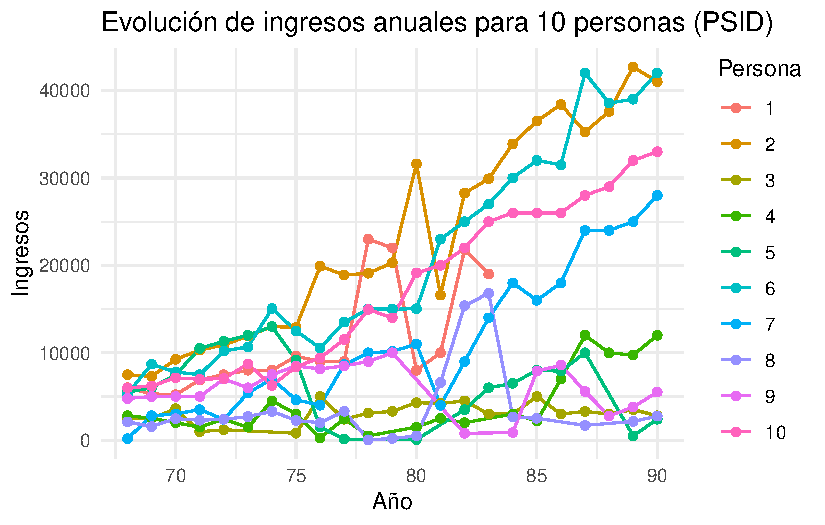
\includegraphics{cap2_files/figure-pdf/unnamed-chunk-1-1.pdf}

\textbf{Figura 1}. Evolución de los ingresos anuales de 10 personas a lo
largo del tiempo.

La figura 1 muestra la evolución de los ingresos anuales para diferentes
personas a lo largo del tiempo, en el que cada línea representa a una
persona.

Esto permite mostrar cómo los ingresos varían entre individuos y años,
observando que los datos son heterogéneos y varían significativamente
entre individuos. Sin embargo, dentro de cada individuo, los ingresos en
un año determinado tienden a ser similares a los del año anterior y el
siguiente, lo que sugiere una correlación temporal en las mediciones.
Esta dependencia entre observaciones dentro de cada individuo es una
característica fundamental de los datos longitudinales, ya que implica
que el valor de la variable en un momento dado está influenciado por
valores previos del mismo individuo; algo que viola los supuestos
básicos de independencia de las observaciones, fundamentales para
modelos clásicos como la regresión lineal simple.

Visto esto, modelaremos la relación entre los ingresos y el tiempo
utilizando una regresión lineal simple, ignorando la dependencia entre
observaciones.

La figura 2 muestra el ajuste de la regresión lineal simple aplicada a
los datos:

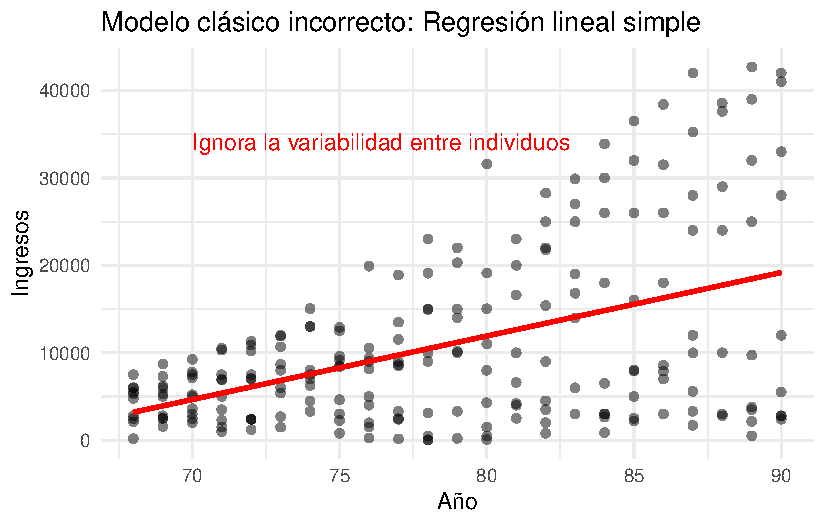
\includegraphics{cap2_files/figure-pdf/unnamed-chunk-3-1.pdf}

\textbf{Figura 2}. Ajuste de un modelo de regresión lineal simple a los
datos observados. La línea roja representa la pendiente estimada, que
asume que todos los individuos comparten la misma relación entre
ingresos y tiempo.

Este gráfico muestra cómo la regresión lineal simple aplicada a estos
datos genera una representación distorsionada, ignorando por completo la
correlación de los datos longitudinales; dando lugar a un mal ajuste y a
resultados estadísticos inapropiados que demuestran por qué no debemos
utilizar estadística clásica para este tipo de datos. No obstante, vamos
a analizar la adecuación y diagnóstico del modelo para ver realmente
cómo las técnicas de estadística clásica no son las correctas para
trabajar con datos longitudinales.

Ya solo al utilizar un modelo de regresión lineal simple, estamos
asumiendo que la variabilidad entre individuos se puede representar con
un único coeficiente, ignorando por completo la dependencia entre
observaciones. Para evaluar la adecuación del modelo, fijémonos en una
medida de bondad de ajuste como el coficiente de determinación R². El R²
obtenido (\textbf{0.217}) es muy bajo, indicando que el modelo explica
muy poca variabilidad en los datos (21\%) y que, por tanto, no nos sirve
para analizar datos longitudinales ya que no captura adecuadamente la
relación entre las variables.

Para realizar el diagnóstico del modelo, haremos un análisis de los
residuos del modelo. Recordemos que dicho análisis se basa en 4 partes
fundamentales: la normalidad de los residuos, que tengan media cero, la
no correlación y la homocedasticidad.

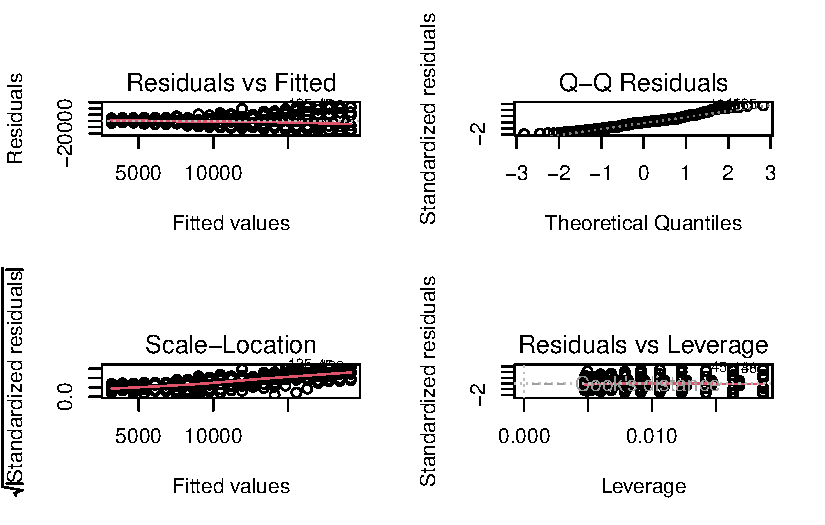
\includegraphics{cap2_files/figure-pdf/unnamed-chunk-5-1.pdf}

\textbf{Figura 3}. Gráficas de los residuos del modelo.

Primero de todo, analicemos la \textbf{normalidad} de los residuos. Para
ello, nos fijamos en la gráfica superior derecha (Normal Q-Q), en la
cual vemos que aunque la mayoría de los puntos se alinean con la línea
teórica, no son pocas las desviaciones que hay en los extremos; lo que
sugiere que los residuos no son perfectamente normales. Para salir de
dudas, podemos aplicar un test de Jarque Bera. El test de Jarque Bera
comprueba si los residuos siguen una distribución normal evaluando su
asimetría y curtosis. Sus hipótesis son las siguientes: \[
\begin{cases} 
H_0 : \text{Los residuos siguen una distribución normal} \\ 
H_1 : \text{Los residuos no siguen una distribución normal}
\end{cases}
\] Si el p-valor es menor a un umbral significativo (por defecto decimos
que es 0.05), se rechaza la hipótesis nula, indicando que los residuos
no siguen una distribución normal.

A través de este test, el p-valor (\textbf{0.024}) nos permite concluir
que podemos rechazar la hipótesis nula y que, por tanto, los residuos no
tienen normalidad.

Lo segundo que vamos a analizar es la \textbf{media cero} de los
residuos. Su hipótesis de asunción es la siguiente: \[
\begin{cases} 
H_0 : \text{Los residuos tienen una media esperada de 0} \\ 
H_1 : \text{Los residuos no tienen una media esperada de 0}
\end{cases}
\]

Si calculamos la media de los residuos del modelo, comprobamos que la
media es \textbf{0}, pero esta no es una forma correcta de anlizar la
media cero ya que esto no significa que la suposición de media cero se
cumpla en todas partes del rango de los valores ajustados. Para hacer un
correcto análisis, nos vamos a fijar en la primera gráfica: Residuals vs
Fitted. Teóricamente, para que los residuos tengan media cero, deberían
de estar uniformemente dispersos alrededor del eje horizontal en
\(y=0\). Viendo la gráfica, podemos observar que los errores no tienen
media cero ya que para los valores ajustados más altos se alejan mucho
de la recta \(y=0\); por lo que esta es otra muestra más de que el
modelo no es correcto para este tipo de datos.

La tercera parte que vamos a analizar es la \textbf{no correlación}
entre los errores, la cual se puede analizar en la primera gráfica. Si
nos fijamos, se observa un patrón curvilíneo a medida que aumenta el
valor de los valores ajustados, por lo que se podría concluir que los
errores están correlacionados. No obstante, para una verificación
numérica haremos un test de Durbin-Watson para comprobar la no
correlación. El test de Durbin-Watson verifica si los residuos están
correlacionados en el tiempo. Sus hipótesis son las siguientes: \[
\begin{cases} 
H_0 : \text{No hay autocorrelación entre los residuos} \\ 
H_1 : \text{Existe autocorrelación entre los residuos}
\end{cases}
\]

En efecto, haciendo el test de Durbin-Watson vemos como el p-valor
(\textbf{0}) es extremadamente bajo y nos permite concluir que podemos
rechazar la hipótesis nula y, por tanto, asumir que la correlación entre
los errores no es 0; otro motivo más para ver que este modelo no
funciona bien con datos longitudinales.

Por último, analizaremos la \textbf{homocedasticidad} de los errores.
Para ello, nos fijaremos en la primera (Residuals vs Fitted) y en la
tercera gráfica (Scale-Location). A través de la gráfica Residuals vs
Fitted, vemos como los residuos no tienen una varianza constante, sino
que a medida que aumenta el valor de los valores ajustados aumenta su
dispersión; por lo que no tienen homocedasticidad, sino
heterocedasticidad. Mirando la gráfica Scale-Location, podemos observar
una tendencia creciente por parte de los residuos que nos permite ver
cómo no tienen varianza constante. Para confirmarlo, haremos un test de
Breusch-Pagan. El test de Breusch-Pagan evalúa si los residuos presentan
heterocedasticidad; es decir, si su varianza no es constante. Sus
hipótesis son las siguientes: \[
\begin{cases} 
H_0 : \text{Los residuos tienen varianza constante (homocedasticidad)} \\ 
H_1 : \text{Los residuos no tienen varianza constante (heterocedasticidad)}
\end{cases}
\]

De nuevo, vemos cómo el p-valor (\textbf{0}) es extremadamente pequeño,
lo que nos permite rechazar la hipótesis nula y, por lo tanto, concluir
que los residuos no tienen varianza constante.

A través de este análisis, hemos podido comprobar que no podemos usar
modelos de estadística clásica, tal y como la regresión lineal simple,
para trabajar con datos longitudinales.

Una visión más acertada sería utilizar un modelo que se ajuste a cada
individuo.

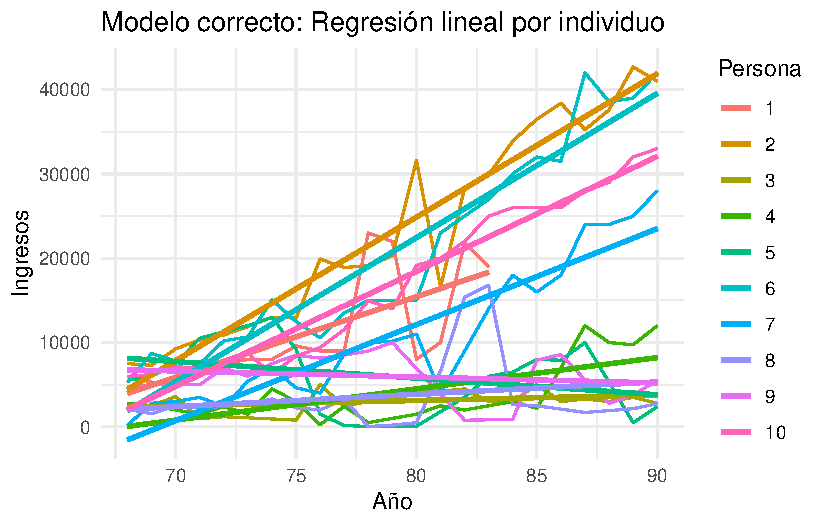
\includegraphics{cap2_files/figure-pdf/unnamed-chunk-10-1.pdf}

\textbf{Figura 4}. Gráfica del modelo para cada individuo.

En esta gráfica, podemos observar que cada individuo tiene un
comportamiento único en cuanto a la evolución de sus ingresos a lo largo
del tiempo. Los interceptos y las pendientes varían considerablemente
entre las personas, lo que evidencia que un único modelo no puede
capturar adecuadamente la relación entre el tiempo y los ingresos para
todos los individuos. Este resultado destaca la heterogeneidad presente
en los datos y la necesidad de utilizar modelos que consideren esta
variabilidad. Al ajustar un modelo por cada individuo, capturamos mejor
las características específicas de cada sujeto, pero esta estrategia
presenta limitaciones: aunque mejora la representación de la
variabilidad entre individuos, no permite hacer inferencias generales
sobre la población; además de que en escenarios con un gran número de
individuos, esta aproximación no es práctica. Por ello, los
\textbf{modelos mixtos} emergen como una solución adecuada, ya que
combinan los llamados efectos fijos y aleatorios para capturar tanto las
tendencias generales de la población como las diferencias específicas
entre individuos. Esta aproximación ofrece un equilibrio entre
flexibilidad y generalización, respetando las características únicas de
los datos longitudinales.

\bookmarksetup{startatroot}

\chapter{Capítulo 3: Modelos mixtos}\label{capuxedtulo-3-modelos-mixtos}

\section{Modelos Lineales Mixtos
(LLM)}\label{modelos-lineales-mixtos-llm}

Son métodos y modelos estadísticos que sirven para analizar datos
longitudinales cuando la variable respuesta sigue una distribución
normal. Se considera la técnica más eficaz cuando se trabaja con
distribuciones normales en este campo ya que permite introducir efectos
aleatorios y concretar la estructura de las correlaciones de los
residuos del mismo sujeto; además de que puede emplearse con datos
faltantes. Estos modelos nos permiten modelar la correlación entre
observaciones dentro de una misma unidad e incluir covariables tanto a
nivel individual como grupal. Permiten realizar una estimación precisa
de la incertidumbre, respetando la dependencia entre observaciones, y la
capacidad de generalización a estructuras de datos complejas son otro de
los motivos por los cuales se recomienda su uso con datos
longitudinales. Otra de sus ventajas es su flexibilidad para incluir
efectos específicos por individuo o grupo; algo que veremos más
adelante.

La ecuación para este tipo de modelos, en los que \(i\) es el individuo
y \(j\) la observación es la siguiente: \[
y_{ij} = \beta_{0i} + \sum_{k=1}^{K} \beta_{ki}x_{ijk} + e_{ij} 
\]

\begin{itemize}
\item
  \(x_{ijk}\) es el valor de la k-ésima variable independiente por parte
  del individuo \(i\) en la observación \(j\).
\item
  \(\beta_{0i}\) sigue \(N(\beta_{0}, \sigma^2_{\beta_{0}})\); es la
  constante del modelo, que suele tener cierta varianza centrada en
  \(\mu\) porque se supone aleatoria.
\item
  \(\beta_{ki}\) sigue \(N(\beta_{k}, \sigma^2_{\beta_{k}})\); son las
  pendientes o coeficientes de las variables independientes del modelo,
  que suelen ser aleatorias.
\end{itemize}

Los \textbf{efectos aleatorios} es el vector formado por la constante y
los coeficientes aleatorios del modelo. Nos permiten capturar la
variabilidad entre individuos, y se escriben de esta forma: \[
\vec{\beta}_i = (\beta_{0i}, \beta_{1i}, \ldots, \beta_{Ki})^t \sim N(\vec{\beta}, \Omega)
\] Cabe destacar que los errores de un individuo, al no tener todos el
mismo número de observaciones, son \textbf{independientes} de los
efectos aleatorios.

Para ajustar un modelo lineal mixto, se tienen que disponer los datos de
forma vertical. Una de las ventajas del LLM es su flexibilidad ya que no
sólo permite especificar efectos aleatorios para evaluar la
\textbf{variabilidad} de algunas variables entre los individuos, sino
que también permite evaluar la \textbf{correlación} entre distintos
datos longitudinales del mismo individuo. La constante y los
coeficientes aleatorios tienen \textbf{homocedasticidad}, ya que la
esperanza y la matriz de covarianzas es la misma para todos los
individuos. Una de las características de los LLM es que introducen el
concepto de \textbf{efectos fijos}, los cuales son la esperanza de los
efectos aleatorios. De hecho, cuando un coeficiente no es aleatorio, se
puede asumir que sigue una distribución normal con varianza cero;
denominándolo fijo. En estos modelos, el número de efectos aleatorios es
limitado, ya que no pueden superar en ningún caso el número de medidas
que tenemos por individuo. Estos efectos inducen una
\textbf{correlación} entre datos para el mismo individuo, pero
dependiendo de su estructura la correlación sólo se puede obtener a
partir de la correlación entre residuos; ya que si consideramos los
coeficientes de variables \textbf{cambiantes} en el tiempo como
aleatorios la correlación es distinta según los tiempos de las medidas,
mientras que si consideramos los coeficientes de variables
\textbf{constantes} en el tiempo inducimos \textbf{heterocedasticidad}
entre individuos.

A la hora de trabajar con Modelos Lineales Mixtos, se puede trabajar de
diferentes formas. Podemos establecer un modelo con la constante
aleatoria y varios coeficientes fijos en el tiempo, en cuyo caso, si
asumimos que los errores son independientes, tendríamos una correlación
\textbf{constante} entre las variables del mismo individuo que no
depende de la distancia entre las medidas; lo que se denomina como
coeficiente de correlación intraclase (ICC). Otra forma de definir estos
modelos podría ser con la constante y los coeficientes aleatorios,
donde, asumiendo independencia entre residuos, la correlación entre
observaciones pasa a depender tanto del tiempo como de la distancia
entre ellas. Sin embargo, pese a ser las dos buenas opciones, es
preferible trabajar de otra forma para LLM.

Para empezar, no asumiremos independencia de los residuos; sino que
trabajaremos con un modelo más general en el que contemos con el mayor
número posible de efectos aleatorios correlacionados y fijos. A
continuación, procederemos a simplificar el modelo a través de la
significación de \textbf{efectos aleatorios}: \[
\begin{cases} 
H_0 : \sigma^2_{\beta_0} = 0 \\ 
H_1 : \sigma^2_{\beta_0} > 0 
\end{cases}
\] Para comprobar que hay más de un efecto aleatorio significativo, se
utilizan diferentes técnicas estadísticas para contrastar que se permite
asumir que podemos rechazar la hipótesis nula: los efectos aleatorios
tienen varianza igual a cero. En caso afirmativo, tenemos que contrastar
que si su correlación es distinta de 0; para lo que tendremos que elegir
la matriz de covarianzas de los efectos aleatorios: \[
\begin{cases}
H_0 : \Omega = 
\begin{pmatrix}
\sigma^2_{\beta_0} & 0 \\
0 & \sigma^2_{\beta_1}
\end{pmatrix} \\
H_1 : \Omega = 
\begin{pmatrix}
\sigma^2_{\beta_0} & \sigma_{\beta_0 \beta_1} \\
\sigma_{\beta_0 \beta_1} & \sigma^2_{\beta_1}
\end{pmatrix}
\end{cases}
\] En este caso, utilizaremos un test de razón de verosimilitudes para
escoger la estructura de covarianzas de los efectos aleatorios y de sus
errores. Para ello, hay que tener en cuenta que los modelos estén
\textbf{anidados}, es decir, que la matriz de covarianzas de los
residuos de un modelo se expresen como un caso particular de la matriz
de covarianzas de los residuos del otro modelo.

Una vez hemos terminado con los efectos aleatorios, procedemos a
determinar la significación de los efectos fijos a través de dos
métodos. Si queremos testear un sólo parámetro, utilizaremos el test de
Wald en el que: \[
\begin{cases}
H_0 : \beta_1 = 0 \\
H_1 : \beta_1 \neq 0
\end{cases}
\] En caso de querer testear más de un parámetro, utilizaremos un test
de razón de verosimilitudes: \[
\begin{cases}
H_0 : \beta_1 = \beta_2 = 0 \\
H_1 : \text{alguno diferente de 0}
\end{cases}
\] Una vez hemos definido ya nuestro modelo, tenemos que realizar su
validación a través de comprobar que se cumplen las asunciones sobre los
residuos; al igual que hacíamos con Regresión Lineal Simple. Para poder
asumir que el modelo es correcto, en el gráfico \textbf{residuos
estandarizados vs valores predichos}, debería de aparecer una especie de
nube de puntos en los que no haya ningún patrón ni ninguna tendencia
aparente; mientras que en el \textbf{QQ-plot}, si los residuos se
encuentran alrededor de la diagonal sin seguir tampoco ningún patrón,
podremos asumir que los residuos tienen normalidad. Para validar lod
efectos aleatorios, podemos utilizar \textbf{Empirical Bayes Estimates}
en lugar de asumir su normalidad.

\section{Modelos Lineales Generalizados
(GLM)}\label{modelos-lineales-generalizados-glm}

Los Modelos Lineales Generalizados son una generalización de los modelos
lineales para una variable respuesta perteneciente a la familia
exponencial, en la que tenemos una función link que describe como la
media de la variable respuesta y la combinación lineal de variables
explicativas están relacionadas.

La \textbf{familia exponencial} suele tener esta forma: \[
f(y \mid \theta, \phi) = \exp \left[ \frac{y\theta - b(\theta)}{a(\phi)} + c(y, \phi) \right]
\] En esta ecuación, \(\theta\) es el \textbf{parámetro canónico} y
representa la posición (location); mientras que \(\phi\) es el
\textbf{parámetro de dispersión} y representa la escala (scale). De la
misma forma, \(a\), \(b\) y \(c\) representan diferentes miembros de la
familia exponencial. En función del parámetro de dispersión, podemos
distinguir entre familias exponenciales de \textbf{un} parámetro, y
familias exponenciales de \textbf{dos} parámetros.

Para determinar si un modelo está basado en un único parámetro
\(\theta\), tenemos que poder escribir su función de probabilidad de la
siguiente forma: \[
f(y; \theta) = e^{[a(y)b(\theta) + c(\theta) + d(y)]}
\] Si el conjunto de posibles valores de entrada no depende de
\(\theta\), la familia exponencial será de un parámetro. Como familias
exponenciales de un parámetro, tenemos las distribuciones de Poisson y
la Binomial. Vamos a demostrar que la distribución de Poisson es, en
efecto, una familia exponencial de un parámetro.

Para ello, aplicando propiedades logarítmicas, podemos definir la
distribución de Poisson como: \[
P(Y = y) = e^{-\lambda} e^{y \log \lambda} e^{-\log(y!)} \\
= e^{y \log \lambda - \lambda - \log(y!)}
\] Si comparamos esta función de masa de probabilidad con la fnción de
probabilidad general para familias con un único parámetro, podemos ver
que: \[
\begin{aligned}
a(y) &= y \\
b(\theta) &= \log(\lambda) \\
c(\theta) &= -\lambda \\
d(y) &= -\log(y!)
\end{aligned}
\] La función \(b(\theta)\) es lo que denominamos \textbf{link
canónico}, una función que nos permite modelar como una función lineal
de variables explicativas.

Como familias exponenciales de dos parámetros, tenemos la distribución
Gamma y la Normal. De forma parecida a la anterior, podemos demostrar
que la distribución Normal es una familia exponencial de dos parámetros.

Podemos definir la función de densidad de una distribución Normal como:
\[
f(y | \mu, \sigma^2) = \frac{1}{\sqrt{2\pi\sigma^2}} \exp \left( -\frac{(y - \mu)^2}{2\sigma^2} \right)
\] Si separamos términos y los escribimos como términos logarítmicos,
tenemos que: \[
f(y | \mu, \sigma^2) = \exp \left( y \cdot \frac{\mu}{\sigma^2} - \frac{y^2}{2\sigma^2} + \left( -\frac{\mu^2}{2\sigma^2} - \frac{1}{2} \log(2\pi\sigma^2) \right) \right)
\] Si comparamos esta función de densidad con la forma general de la
familia exponencial, podemos ver que: \[
\begin{aligned}
a(y) = y\\
b(\mu, \sigma^2) = \frac{\mu}{\sigma^2}\\
c(\mu, \sigma^2) = -\frac{\mu^2}{2\sigma^2} - \frac{1}{2} \log(2\pi\sigma^2)\\
d(y, \sigma^2) = -\frac{y^2}{2\sigma^2}\\
\end{aligned}
\] Por lo tanto, demostramos que la distribución normal también
pertenece a la familia exponencial, pero con una peculiaridad respecto a
la distribución de Poisson: es una familia exponencial de dos
parámetros, la media \(\mu\) y la varianza \(\sigma^2\). En este caso,
el término \(b(\mu, \sigma^2)\) es el \textbf{link canónico} que conecta
las variables explicativas con el modelo.

En concreto, para los casos en los que la respuesta no es normal, la
ecuación del modelo es la siguiente: \[
g\left(E(y_{ij} \mid x_{ijk}, \beta_{0i}, \dots, \beta_{Ki})\right) = \beta_{0i} + \sum_{k=1}^{K} \beta_{ki}x_{ijk}
\] Donde g es la función link y, pese a que puede parecerse mucho a la
función para modelos LMM, tienen algunas diferencias, como que en el
primer miembro tenemos el link del valor esperado en vez de la variable
respuesta, y en el segundo miembro no se cuenta con los errores; por lo
que no existe una matriz de correlaciones de los residuos. De esta
forma, ya hemos \textbf{generalizado} nuestro modelo para manejar
variables respuesta que no siguen una distribución normal. A través de
esta generalización, somos capaces de escribir la función de masa o
densidad de probabilidad de distintas distribuciones para poder modelar
el link canónico como función lineal de las variables predictoras.

\bookmarksetup{startatroot}

\chapter*{Referencias}\label{referencias}
\addcontentsline{toc}{chapter}{Referencias}

\markboth{Referencias}{Referencias}

\phantomsection\label{refs}
\begin{CSLReferences}{0}{1}
\end{CSLReferences}



\end{document}
